\chapter{\uppercase{Neutrino Oscillation in the PROSPECT AD}}

\section{Detecting Antineutrinos}

PROSPECT detects $\bar{\nu_e}$'s via the inverse beta decay reaction (IBD):
\begin{equation}
	\bar{\nu_e} + p \rightarrow e^+ + n
\end{equation}
A reactor $\bar{\nu_e}$ will interact with a proton in the $^6$Li-LS, producing a positron and a neutron.
The positron will quickly lose energy and annihilate with an electron, producing two 511 keV $\gamma$-rays.
This is the prompt signal.

Concurrently, the neutron will thermalize by scattering off of protons in the scintillator until it captures on $^6$Li ($\sim$80\% of the time) or H ($\sim$20\% of the time).
The neutron capture on $^6$Li (nLi) produces a tritium and an alpha with energies 2.05 MeV and 2.75 MeV respectively. 
These two products will immediately scintillate, and produce a quenched signal of $\sim$0.55 MeVee.
This is the delayed signal.
Figure~\ref{fig:ibd} illustrates this process in the PROSPECT LiLS.

The neutron capture on $^6$Li takes $\sim$40$\mu$s, providing a time separation between the prompt and delayed signals.
Making use of the time coincident, PSD, and energy cuts, PROSPECT can identify $\bar{\nu_e}$ events above background. 

\begin{figure}[!t]
	\centering
	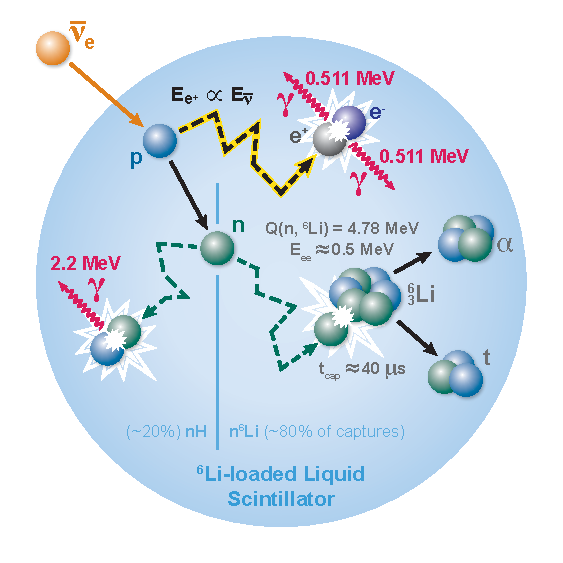
\includegraphics[width=0.4\linewidth]{tex/7-oscillation-images/IBD}
	\caption{Schematic of the IBD interaction is the PROSPECT AD.}
	\label{fig:ibd}
\end{figure}

\section{IBD Event Selection}

\subsection{Cuts}

A selection of energy, PSD, and time cuts, along with specified event vetos are utilized to identify IBD signals and reduce background.
These are:
\begin{itemize}
	\item Prompt Cluster Size: $\geq1$
	\item Prompt PSD: All pulses must have PSD that is $<3\sigma$ from the gamma-like PSD band mean
	\item Prompt Energy: No cut, but only clusters with a total energy of 0.8 $<$ E$_{\textrm{rec}} <$ 7.2 MeV are used in the oscillation analysis
	\item Delayed Cluster Size: Single pulse
	\item Delayed PSD: All pulses must have PSD that is $>3.6\sigma$ from the gamma-like PSD band mean
	\item Delayed Energy: 0.46 $<$ E$_{\textrm{rec}} < $0.60 MeV
	\item Time Correlation: $\Delta t = (1,120)~\mu$s
	\item Prompt-Delayed Distance: $\Delta z <$ 18 cm for coincidences in the same segment; $\Delta z <$ 14 cm for coincidences in horizontally/vertically adjacent segments
	\item Pileup Veto: Applied to both prompt and delayed clusters, if the candidate cluster is preceded by another cluster in a window of $<$ 800 ns, the candidate cluster is vetoed
	\item Shower Veto: Veto delayed clusters that exist in a (0,100) $\mu$s window around cosmic muon clusters (E$_{\textrm{rec}} >$ 15 MeV); Veto delayed clusters that exist within (-200,+200)~$\mu$s of events with PSD $> 3\sigma$ from the gamma-like PSD band mean and E $>$ 0.25 MeV
	\item Fiducialization: Reject events in which a prompt or delayed event occurs in the outer ring of segments; reject events that occur outside of $z$ = (-448, 448) mm 

\end{itemize}

\subsection{Backgrounds}



\section{Data Set}
\begin{figure}[H]
	\centering
	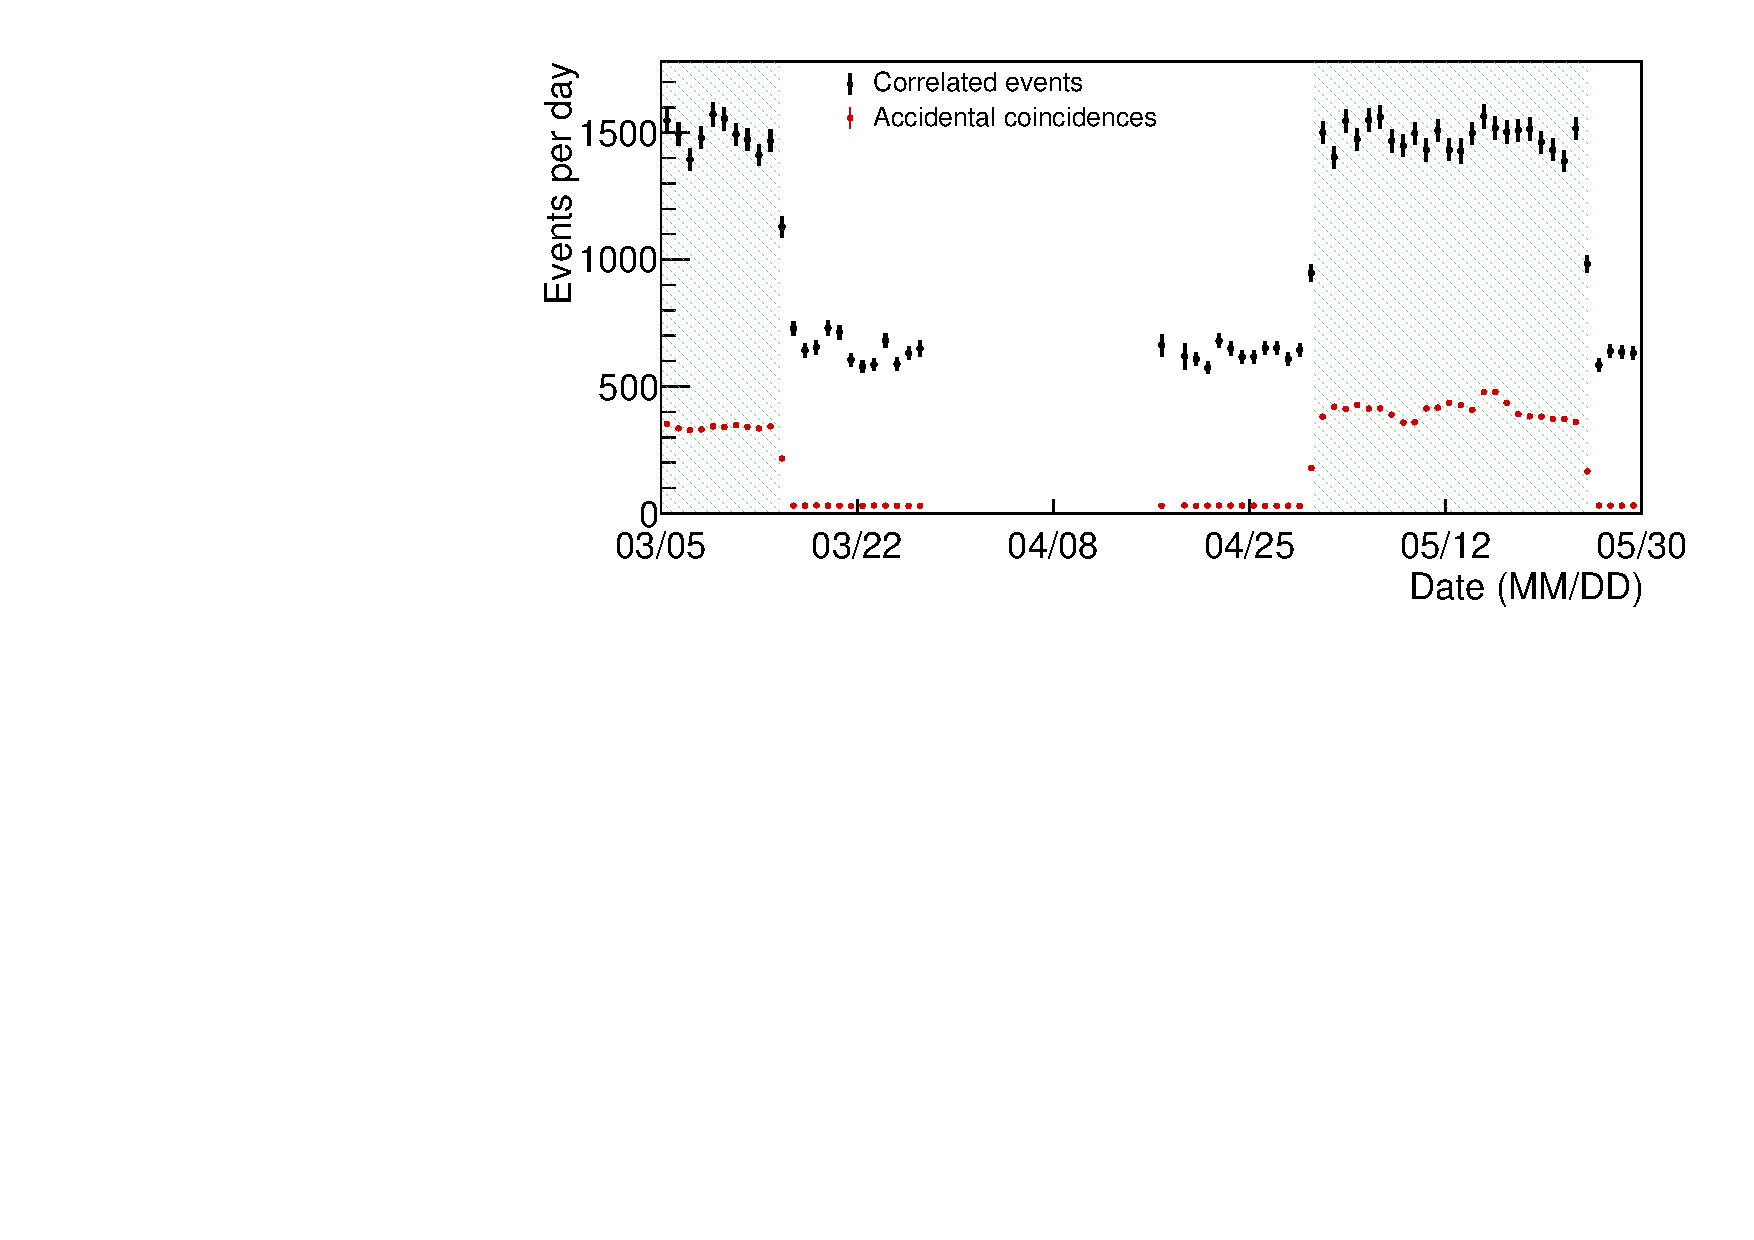
\includegraphics[width=0.7\linewidth]{tex/7-oscillation-images/EvtRates}
	\caption{}
	\label{fig:evtrates}
\end{figure}



\noindent Background:
\begin{itemize}
	\item Cosmogenics
	\item Atmospheric correction
	\item Background subtraction
\end{itemize}

\begin{figure}[H]
	\centering
	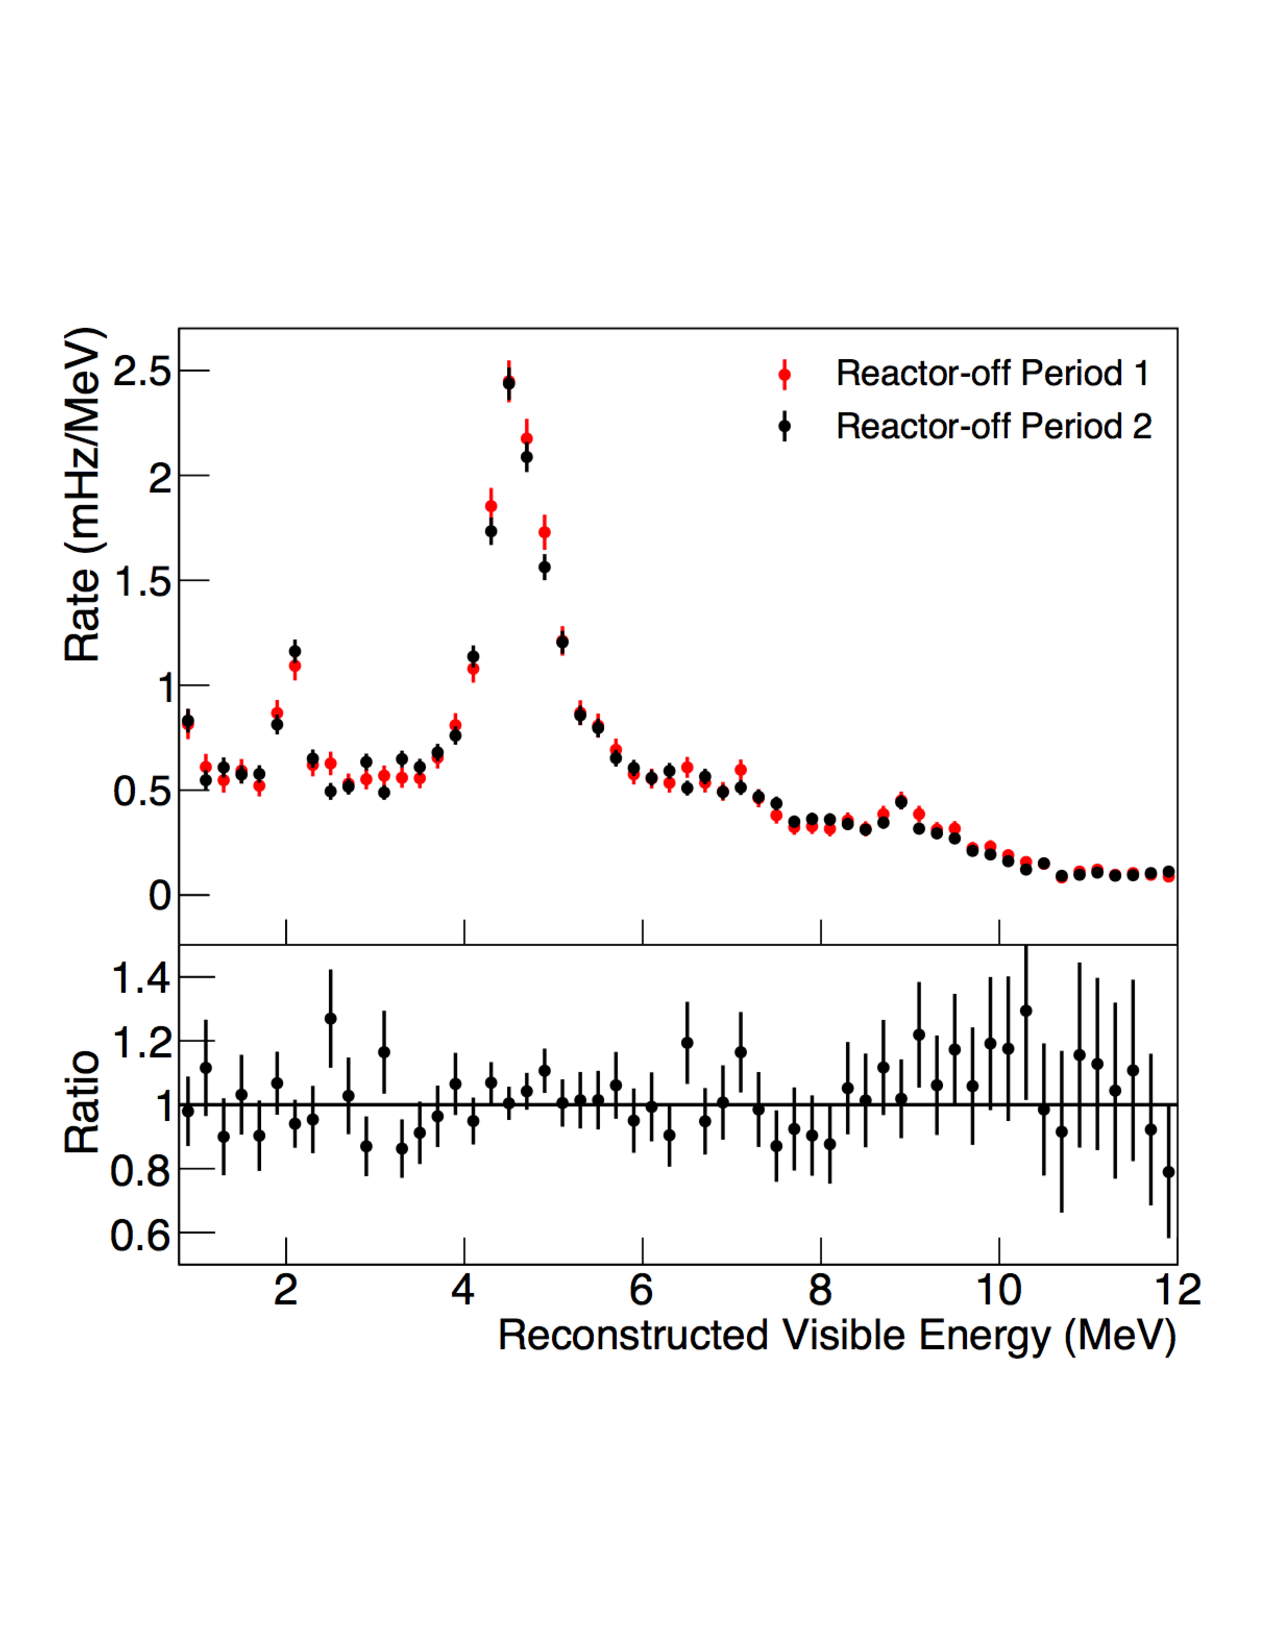
\includegraphics[width=0.7\linewidth]{tex/7-oscillation-images/RxOffSpectrum}
	\caption{}
	\label{fig:rxoffspectrum}
\end{figure}



\begin{figure}[H]
	\centering
	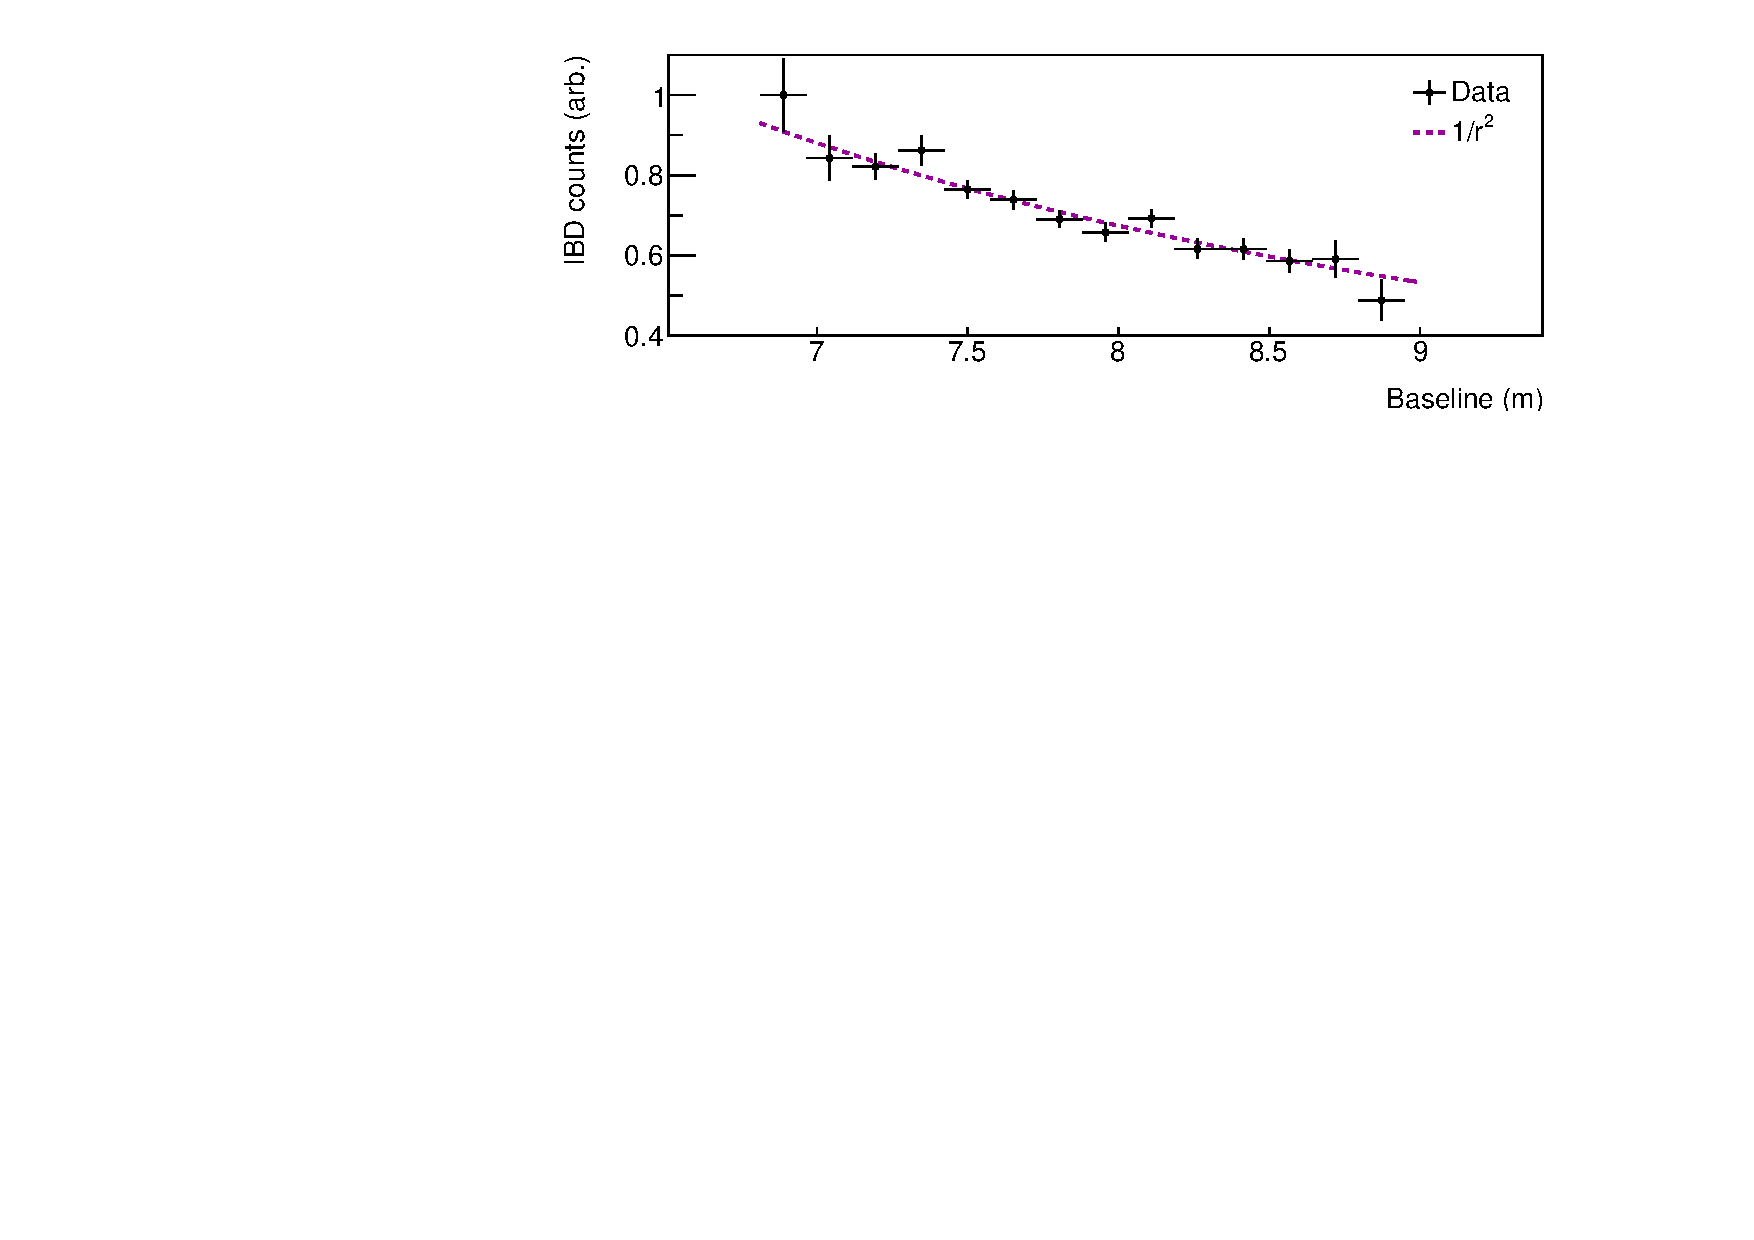
\includegraphics[width=0.7\linewidth]{tex/7-oscillation-images/IBDvsBaseline}
	\caption{}
	\label{fig:ibdvsbaseline}
\end{figure}



\section{Oscillation Results}

\begin{figure}[H]
	\centering
	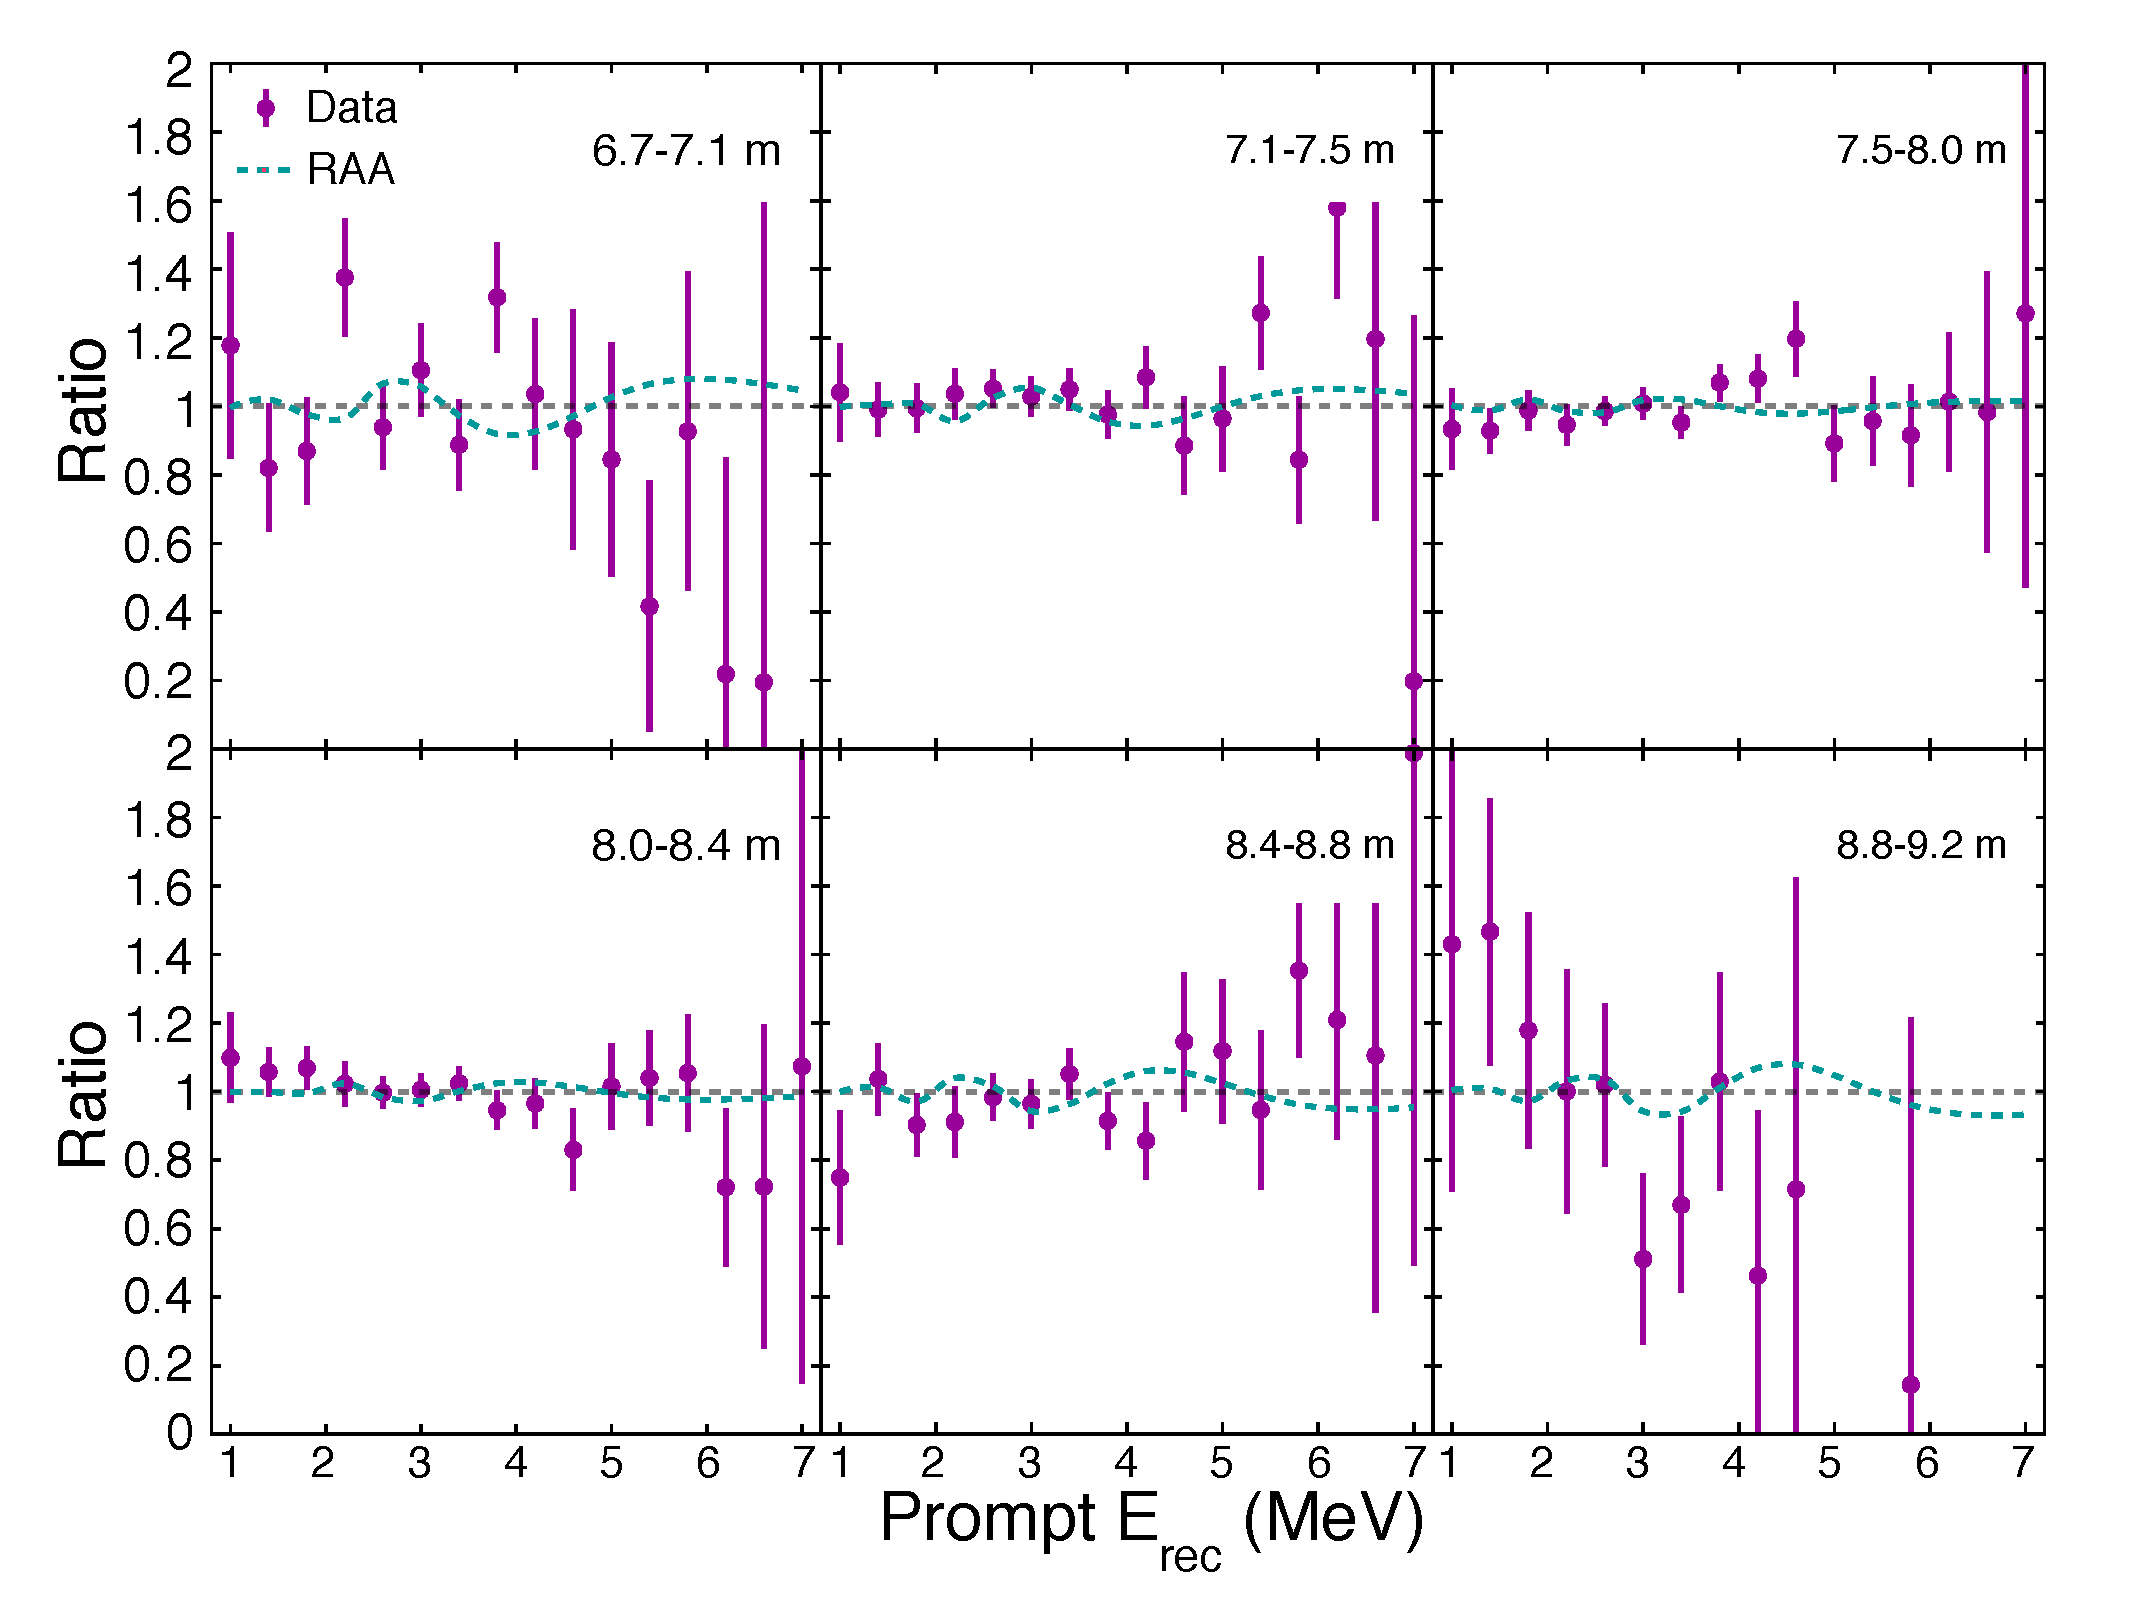
\includegraphics[width=0.7\linewidth]{tex/7-oscillation-images/BaselineSpectra}
	\caption{}
	\label{fig:baselinespectra}
\end{figure}

\begin{figure}[H]
	\centering
	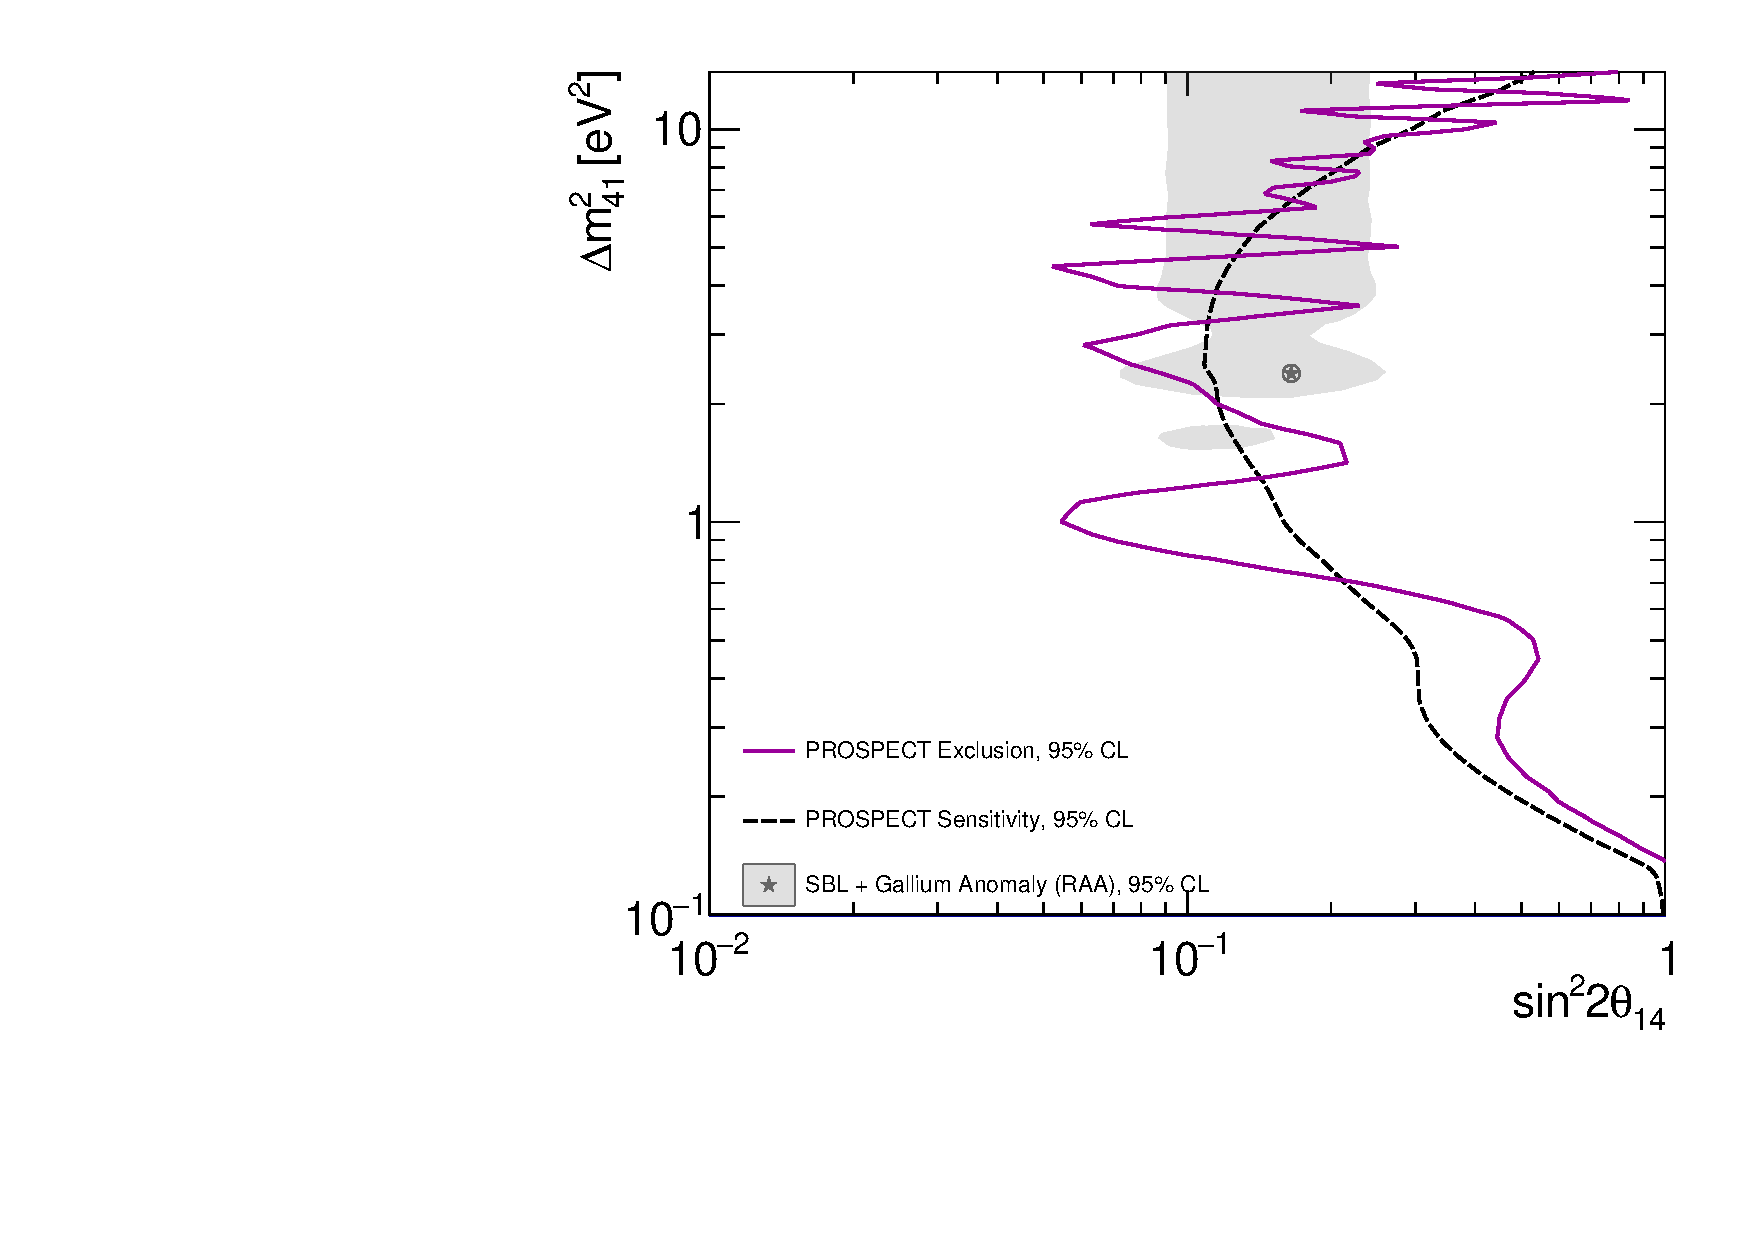
\includegraphics[width=0.7\linewidth]{tex/7-oscillation-images/Exclusion_Sensitivity_Final}
	\caption{}
	\label{fig:exclusionsensitivityfinal}
\end{figure}



\section{Spectrum Results}
\begin{figure}[H]
	\centering
	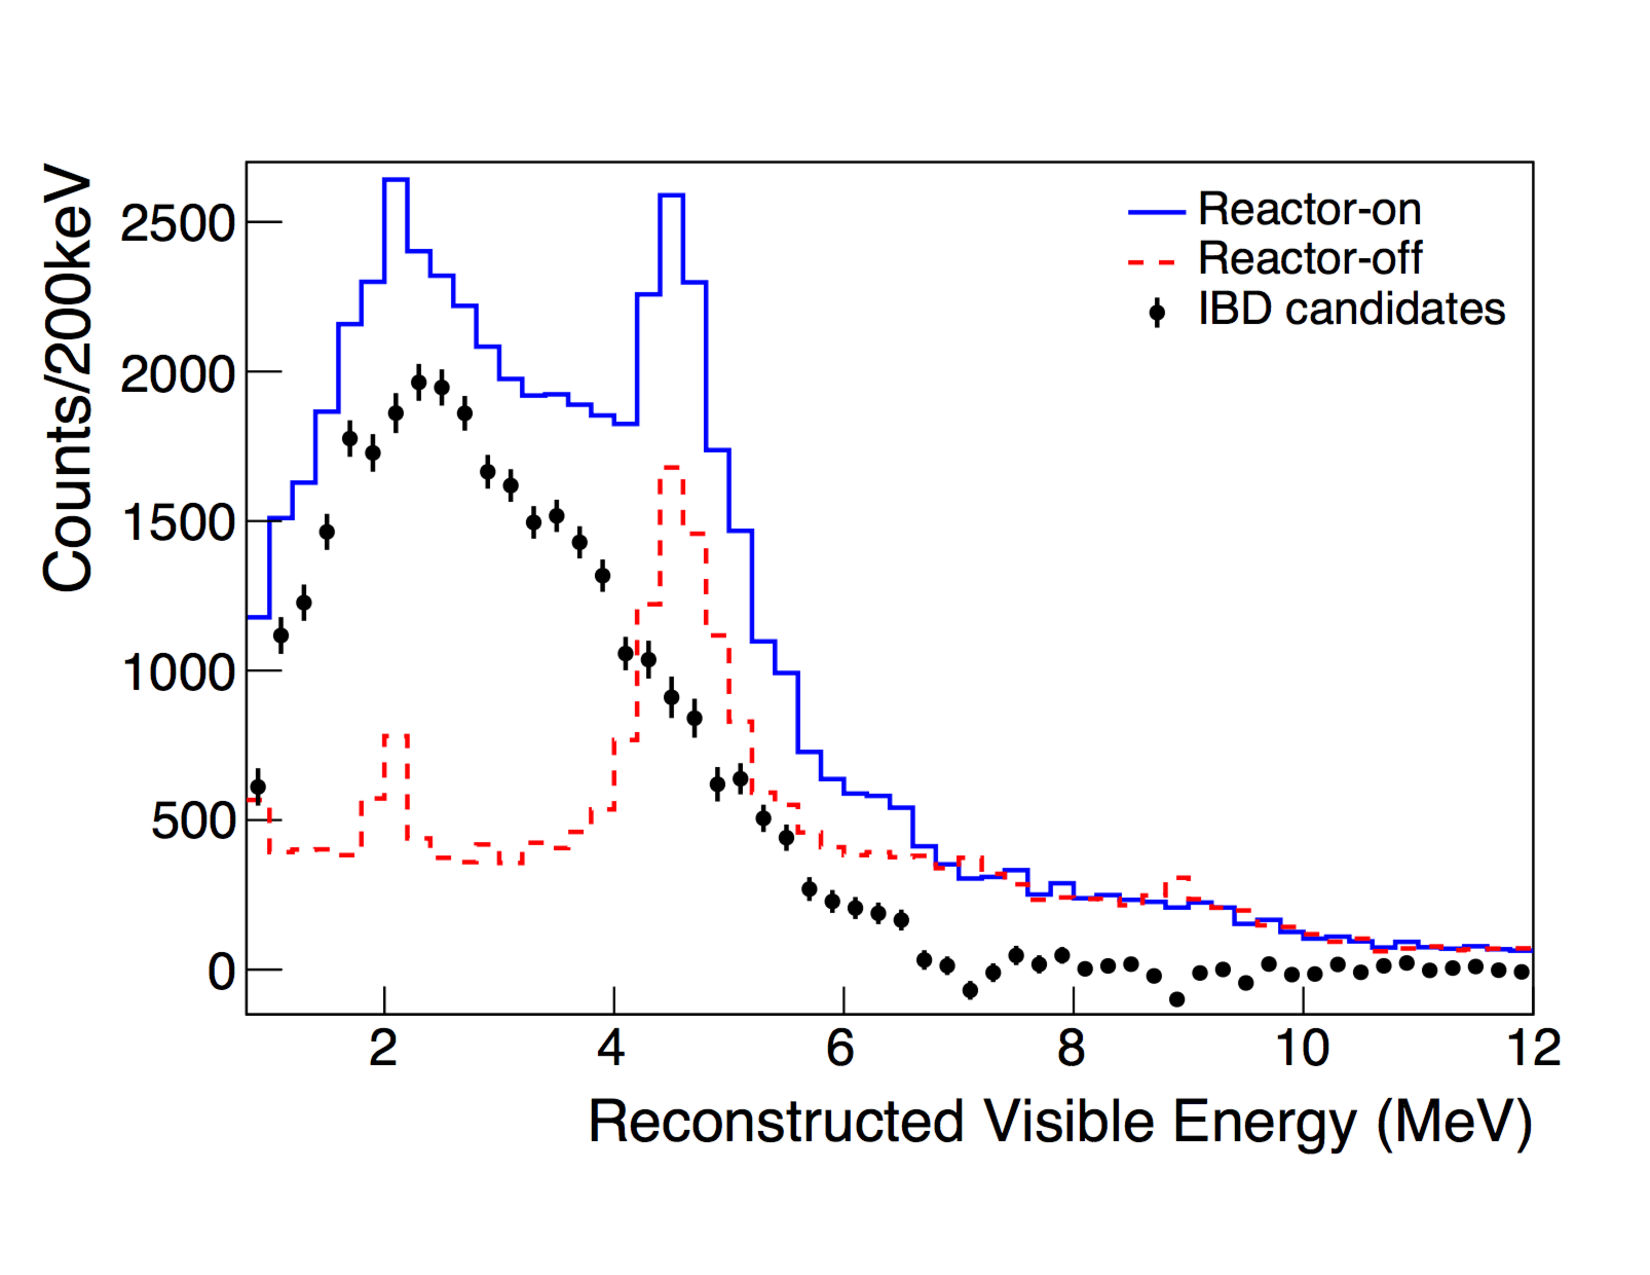
\includegraphics[width=0.7\linewidth]{tex/7-oscillation-images/Spectrum}
	\caption{}
	\label{fig:spectrumresults}
\end{figure}



